\documentclass[11pt,a4paper]{article}

% Packages
\usepackage[utf8]{inputenc}
\usepackage[T1]{fontenc}
\usepackage{amsmath,amssymb,amsthm}
\usepackage{graphicx}
\usepackage{hyperref}
\usepackage{booktabs}
\usepackage{xcolor}
\usepackage[margin=2.5cm]{geometry}
\usepackage[numbers]{natbib}
\usepackage[protrusion=true,expansion=false]{microtype}

% Theorem environments
\newtheorem{theorem}{Theorem}[section]
\newtheorem{lemma}[theorem]{Lemma}
\newtheorem{proposition}[theorem]{Proposition}
\newtheorem{corollary}[theorem]{Corollary}
\newtheorem{definition}[theorem]{Definition}

% Title
\title{Structural Collapse as Information Loss:\\
The Exponential Decay Mechanism under Accumulating Constraints}
\author{Akihito Sunagawa\thanks{akihito.sunagawa@gmail.com}}
\date{March 2026}

\begin{document}

\maketitle

\begin{abstract}
Large language models exhibit abrupt reasoning collapse when structural contradictions accumulate in their context---a phenomenon distinct from gradual degradation under factual noise. Through controlled experiments (11 models, 5 vendors, 4B--70B+ parameters), we characterize this collapse and find: (i) multiplicative interaction between context margin ($\mu$) and structural contradiction ($\delta$)---two individually non-lethal stressors become lethal in combination, ruling out additive degradation models; (ii) a dimensional structure in $\delta$ where, in models with sufficient baseline accuracy, a single structural contradiction causes more damage than 10 factual contradictions; and (iii) a cushion mechanism where RLHF alignment absorbs contradictions until overwhelmed, producing a system-specific critical threshold $\delta_c$.

These patterns are explained by the first moment method from combinatorics. Defining cumulative information loss $\delta = \sum_i I(\text{constraint}_i)$ in nats, we show that the multiplicative survival potential
\[
S = N_{eff} \cdot \frac{\mu}{\mu_c} \cdot e^{-\delta}
\]
captures both the LLM collapse patterns and, in Boolean satisfiability (SAT) where $\delta$ is exactly computable, yields parameter-free predictions: the decay rate ratio $\alpha_{\text{XOR}}/\alpha_{\text{random}} = \ln 2 / |\ln(7/8)| = 5.19\times$ is an upper bound confirmed experimentally (observed: $5.04 \pm 0.25$, CV $= 5\%$; the systematic shortfall is consistent with inter-constraint correlations reducing effective information loss---overlapping constraints create redundancy, so that a single violation's impact on the overall system is mitigated). The exponential penalty $e^{-\delta}$ is not an approximation but a mathematical identity with the first moment of the SAT solution count. Its contribution is an operational methodology---measuring structural conflict as information loss in nats via the first moment correspondence---validated in two controlled domains. Extension to the second moment method (Paley--Zygmund inequality) with pair correlation function $g(\beta) = 3/4 + (1/8)(1-\beta)^3$ quantitatively explains 74\% of the gap between the first-moment upper bound ($\alpha \approx 5.19$) and the true 3-SAT threshold ($\alpha \approx 4.27$); the remaining 26\% is attributable to replica symmetry breaking. All results---including the second moment overlap decomposition---are machine-verified in Lean~4 (15 modules, 152 propositions, no \texttt{sorry}, no axiom).

\medskip
\noindent\textbf{Keywords:} LLM reasoning collapse, structural contradiction, information loss, multiplicative model, SAT phase transition, survival analysis, formal verification
\end{abstract}

%=============================================
\section{Introduction}

Large language models can reason---until they suddenly cannot. In models with sufficient baseline accuracy, a single structural contradiction (a self-referential paradox, a meta-level inconsistency) causes more damage than ten factual contradictions (Section~\ref{sec:llm-delta-structure}). Two individually harmless stressors (moderate context load and moderate contradiction) become lethal in combination (Section~\ref{sec:llm}). These patterns, replicated across eleven models from five vendors spanning 4B to 70B+ parameters (Section~\ref{sec:cross-model}), cannot be explained by additive degradation models such as attention decay or error propagation, both of which predict performance loss proportional to each stressor independently. The phenomenon is distinct from---though related to---model collapse under recursive training data \citep{shumailov2024}, where cumulative information loss manifests as distributional narrowing rather than reasoning failure.

Why multiplicative, not additive? This paper proposes that the answer lies in a well-known mathematical structure: the first moment method from combinatorics. We define the \textbf{cumulative information loss} $\delta = \sum_i I(\text{constraint}_i)$, measured in nats, where each structural constraint contributes a calculable amount of information loss. The survival potential is then:
\begin{equation}
S = N_{eff} \cdot \frac{\mu}{\mu_c} \cdot e^{-\delta}
\label{eq:survival}
\end{equation}
where $N_{eff}$ is the number of effective options (independent alternatives available to the system), $\mu/\mu_c$ is the margin relative to a critical threshold, and $e^{-\delta}$ is the exponential penalty from accumulated structural conflicts. This multiplicative structure---where any factor approaching zero is fatal regardless of the others---is the structure of serial reliability \citep{barlow1975}, nuclear reactor criticality \citep{duderstadt1976}, and epidemic thresholds ($R_0$). Notably, an analogous separation has been institutionalized independently in credit assessment: major rating agencies (S\&P, Moody's, Fitch) distinguish quantitative financial health ($\mu$) from qualitative governance factors ($\delta$), with Moody's explicitly separating ``ability to pay'' from ``willingness to pay''---a capacity--constraint decomposition arrived at through decades of practice without theoretical motivation \citep{cantor1996}.

The contribution is not the multiplicative structure itself, but the information-theoretic grounding: defining $\delta$ operationally in nats via the first moment method, so that constraint quality---not merely quantity---becomes calculable from first principles. In Boolean satisfiability (SAT), $e^{-\delta}$ is mathematically identical to the first moment of the solution count (Section~\ref{sec:first-moment}). This identity yields parameter-free predictions: XOR constraints should cause collapse at $\ln 2 / \ln(8/7) \approx 5.19$ times lower density than random clauses---confirmed experimentally at $5.04 \pm 0.25$ (CV $= 5\%$; Section~\ref{sec:sat}). The same mathematical structure explains why structural contradictions in LLMs are qualitatively more damaging than factual noise: they carry higher information loss per constraint.

\subsection{Research Questions}

\begin{enumerate}
    \item \textbf{Operational definition}: Can structural conflict be measured as information loss ($\delta$ in nats) with a precise correspondence to established mathematics?
    \item \textbf{Multiplicative structure}: Do $N_{eff}$, $\mu/\mu_c$, and $e^{-\delta}$ combine multiplicatively (as in serial reliability), or additively?
    \item \textbf{Prediction}: Does the framework generate parameter-free, falsifiable predictions that hold in controlled experiments?
\end{enumerate}

\subsection{Two Levels of Precision}

We distinguish two levels of applicability:

\begin{itemize}
    \item \textbf{Level~A} (externally defined survival): Systems where survival is defined independently of the system itself and $\delta$ is directly computable. SAT instances (satisfiability) and LLM experiments (correct answer production) operate at this level. Predictions are quantitatively sharp.

    \item \textbf{Level~B} (self-defining survival): Systems where the survival condition depends on the system's own identity and $\delta$ requires proxy measurement. Corporations, organisms, and ecosystems operate at this level. Predictions are approximate, degrading with measurement error $\varepsilon$ as formally bounded by $|S(\delta_{\text{meas}}) - S(\delta_{\text{true}})| \leq N_{eff} \cdot \varepsilon \cdot (\mu/\mu_c)$.
\end{itemize}

This paper focuses on Level~A evidence (SAT experiments and LLM experiments), where $\delta$ is exactly or near-exactly computable.

\subsection{Why Two Domains}

Neither domain alone suffices. SAT validates the $e^{-\delta}$ component---the mathematical identity between cumulative information loss and the first moment of the solution count---but cannot test the multiplicative interaction between $\mu$ and $\delta$, because margin is not a variable in SAT. LLM experiments confirm multiplicative $\mu \times \delta$ interaction and reveal that constraint quality dominates quantity, but cannot independently verify the exponential form (the low-$\delta$ regime does not discriminate $e^{-\delta}$ from $(1-\delta)^k$). The two domains are therefore complementary: SAT anchors the mathematics, LLM anchors the multiplicative structure. Crucially, the epistemic status differs: in SAT, $e^{-\delta}$ is a \emph{mathematical identity} with the first moment (Section~\ref{sec:first-moment}); in LLM, the same functional form is a \emph{structural analogy}, empirically tested rather than derived from first principles. This distinction is developed in Section~\ref{sec:discussion}.

\subsection{Paper Structure}

Section~\ref{sec:related} positions the work relative to prior frameworks. Section~\ref{sec:theory} develops the theoretical framework: the survival equation, the first moment correspondence, and the exponential penalty derivation. Section~\ref{sec:sat} presents SAT experiments with three constraint types and parameter-free predictions. Section~\ref{sec:llm} reports controlled LLM experiments confirming multiplicative structure and the cushion mechanism. Section~\ref{sec:discussion} discusses scope, limitations of the exponential form, and directions for future work. Section~\ref{sec:limitations} details specific limitations. Section~\ref{sec:conclusion} concludes.

%=============================================
\section{Related Work}
\label{sec:related}

\subsection{Survival Analysis and Hazard Models}

The Cox proportional hazards model \citep{cox1972}, building on the Kaplan--Meier estimator \citep{kaplan1958}, establishes the standard framework for survival analysis: $h(t) = h_0(t) \exp(\beta' X)$. Our model shares the exponential form but differs in a key respect: the Cox model treats covariates as post-hoc correlates discovered through regression, while our framework derives the exponential penalty $e^{-\delta}$ from the first moment method in combinatorics, providing a structural interpretation of the exponent.

\subsection{Threshold Phenomena and Early Warning Signals}

Scheffer et al.\ \citep{scheffer2009} established that many complex systems exhibit critical transitions preceded by early warning signals (increased autocorrelation, variance, flickering). May \citep{may1972} showed that ecosystem stability depends on the relationship between diversity and connectivity. Our framework formalizes one mechanism underlying such transitions: the multiplicative accumulation of structural conflicts drives the system toward a critical threshold, with the exponential $e^{-\delta}$ capturing the nonlinear sensitivity to accumulated conflicts.

\subsection{Dissipative Structures}

Prigogine \citep{prigogine1984} established that open systems far from equilibrium maintain structure through continuous energy and information flow. Our survival equation applies to such dissipative structures: the three factors ($N_{eff}$, $\mu/\mu_c$, $e^{-\delta}$) decompose the conditions under which a dissipative structure maintains itself against entropic decay.

\subsection{Information-Theoretic Approaches}

Shannon's channel coding theorem \citep{shannon1948,cover2006} establishes that reliable communication requires redundancy exceeding the channel's noise rate. The first moment method in combinatorics \citep{alon2016} uses $\mathbb{E}[X] = 0 \implies \Pr[X > 0] = 0$ to prove non-existence. Our operational definition $\delta = \sum_i I(\text{constraint}_i)$ connects these: each constraint removes information (solutions, options, capacity), and $e^{-\delta}$ is the expected fraction remaining---exactly the first moment bound.

In the SAT context, Cocco and Monasson \citep{cocco2001} analytically derived the branching rate $\omega(\alpha)$ for DPLL-class solvers, showing that algorithmic cost diverges exponentially near the satisfiability threshold. Their analysis demonstrates that constraint density governs both solvability and computational cost---a connection we formalize through $\delta$ in the companion paper \citep{sunagawa2026sat}. Ben-Sasson and Wigderson \citep{bensasson2001} proved that resolution proof length grows exponentially for random 3-SAT near the threshold, establishing the proof-complexity foundation for why structured solvers (CDCL) cannot avoid exponential cost in the worst case.

In molecular biology, Eigen's error catastrophe \citep{eigen1971} established an information-theoretic threshold for self-replicating systems: when the mutation rate exceeds a critical value, sequence information is irreversibly lost. The threshold condition is formulated in nats, making it structurally isomorphic to our $\delta_c$. The key difference is that Eigen's $\delta$ arises from stochastic copying errors in a single domain (RNA replication), whereas our framework addresses deterministic structural contradictions and is validated across two structurally distinct domains.

Independently, Giannakopoulos \citep{giannakopoulos2025} proposed an exponential survival equation $S(\eta) = \exp[-\alpha \cdot (1-\eta) \cdot Q/T]$ from a different starting point (preprint, not yet peer-reviewed).

\subsection{LLM Reasoning Collapse}

Zhang et al.\ \citep{zhang2026lpt} independently discovered that LLM logical reasoning exhibits abrupt phase transitions---performance remains stable within complexity ranges and then collapses sharply, a phenomenon they term ``logical phase transitions'' (LPT). Their Logical Complexity Metric (LoCM) quantifies task difficulty via weighted operator counts, nesting depth, and inference hops, and the phase transition pattern is observed across 12+ models from multiple vendors.

Our work differs primarily in grounding: our $\delta = \sum_i I(\text{constraint}_i)$ is measured in nats via the first moment correspondence, whereas LoCM uses empirically calibrated weights without a connection to information loss. This nats-based framework enables cross-domain application (SAT, LLM, and in principle organisational and ecological systems) under a single metric.

Independently, Apple ML Research \citep{apple2025illusion} demonstrated that both standard and reasoning-enhanced LLMs exhibit sharp accuracy collapse above a complexity threshold in controlled puzzle environments, identifying three regimes (standard-LLM-dominant, reasoning-model-dominant, and universal collapse). Their work provides independent confirmation of the collapse threshold phenomenon without an information-theoretic framework for its mechanism.

%=============================================
\section{Theoretical Framework}
\label{sec:theory}

\subsection{The Survival Equation}

\begin{definition}[Survival Subject]
A survival subject is a system whose continued function requires maintaining internal consistency under accumulating constraints, and that is capable of collapse ($S \to 0$). In this paper: SAT instances (where collapse $=$ unsatisfiability) and LLM reasoning sessions (where collapse $=$ failure to produce correct answers). The formalism extends in principle to other constraint-processing systems (organisms, organisations, ecosystems), but such extensions require domain-specific $\delta$ calibration and are not validated here.
\end{definition}

The survival potential $S$ is:
\begin{equation}
S = N_{eff} \cdot \frac{\mu}{\mu_c} \cdot e^{-\delta}
\label{eq:survival-main}
\end{equation}

\textbf{$S$ is a potential, not a probability.} The survival potential $S$ is an unnormalized quantity that can exceed 1 when $N_{eff} \cdot (\mu/\mu_c) > 1$. The survival condition is $S > S_c$ (a domain-specific critical threshold), not $S \in [0,1]$. In specific domains, $S$ is related to observable quantities through domain-specific normalization: in SAT, $S/N_{eff} = \mathbb{E}[\#\text{SAT}]/2^n \in [0,1]$ is the normalized expected solution count; in LLM experiments, the accuracy (fraction of correct responses) serves as an empirical proxy for $S/S_{\max}$. These domain-specific observables are bounded, but $S$ itself is not.

The three factors are:
\begin{itemize}
    \item $N_{eff}$ (Effective Options): Number of independent alternatives available to the system. Under OR-gate structure (any alternative suffices), higher $N_{eff}$ improves survival. Under AND-gate structure (all components required), higher $N_{eff}$ increases fragility.
    \item $\mu/\mu_c$ (Margin): The ratio of available resource flow ($\mu$) to the minimum resource flow required for continued function ($\mu_c$). When $\mu/\mu_c > 1$, the system has surplus capacity; when $\mu/\mu_c < 1$, this factor drives $S$ toward zero, though the system may still survive if the other factors compensate. In dissipative structures, $\mu$ and $\mu_c$ are continuous flows, not static stocks---this flow-based definition captures the essential nature of dissipative structures, including LLMs, as dynamic entities that continuously process information to maintain their function. In SAT, this factor is absent.
    \item $e^{-\delta}$ (Structural Integrity): The exponential penalty from cumulative information loss. $\delta = \sum_i I(\text{constraint}_i)$ is measured in nats, where each structural constraint contributes a calculable amount of information loss.
\end{itemize}

\textbf{Multiplicative structure.} The three factors enter as a product, not a sum. This is the structure of serial reliability \citep{barlow1975}: a system with $k$ independent failure modes has survival probability $\prod_i (1 - p_i)$. If any single factor approaches zero, $S \to 0$ regardless of the others. Two individually non-lethal factors can become lethal in combination---a prediction that additive models cannot make, and that we confirm experimentally in Section~\ref{sec:llm}.

\textbf{Independence, not causal chain.} In the static equation, $N_{eff}$, $\mu/\mu_c$, and $\delta$ are independent multiplicative risk factors. In SAT experiments (Section~\ref{sec:sat}), the number of variables ($N_{eff}$) and the clause density ($\delta$) are set independently by the experimenter. In LLM experiments (Section~\ref{sec:llm}), all three factors are independently manipulated. Dynamic feedbacks exist (e.g., accumulated $\delta$ may consume $\mu$ over time), but these are properties of temporal evolution, not of the static equation. The dynamic model is future work.

\subsection{The Exponential Penalty: First Moment Correspondence}
\label{sec:first-moment}

The exponential form $e^{-\delta}$ is not an arbitrary modeling choice. In Boolean satisfiability (SAT), it has a precise mathematical identity.

Consider a random SAT instance with $n$ Boolean variables and $m$ independently generated constraints. Each constraint $C_i$ is satisfied by a fraction $p_i$ of all $2^n$ possible assignments. For a fixed assignment $\sigma$, the events $\{\sigma \text{ satisfies } C_i\}$ are independent because the clauses are generated independently---even if they share variables. By linearity of expectation, the expected number of satisfying assignments is:
\begin{equation}
\mathbb{E}[\#\text{SAT}] = 2^n \prod_{i=1}^{m} p_i = 2^n \prod_{i=1}^{m} (1 - q_i) = 2^n \exp\!\left(\sum_{i=1}^{m} \ln(1 - q_i)\right)
\label{eq:first-moment}
\end{equation}
where $q_i = 1 - p_i$ is the fraction of assignments eliminated by constraint $C_i$.

Define the information loss per constraint:
\begin{equation}
I(C_i) = -\ln(1 - q_i) = -\ln p_i \quad \text{(nats)}
\label{eq:info-loss}
\end{equation}

Then the cumulative information loss is:
\begin{equation}
\delta = \sum_{i=1}^{m} I(C_i)
\label{eq:delta-def}
\end{equation}

and the first moment becomes:
\begin{equation}
\mathbb{E}[\#\text{SAT}] = 2^n \cdot e^{-\delta}
\label{eq:first-moment-exp}
\end{equation}

The survival equation's $e^{-\delta}$ is therefore \emph{identical} to the first moment of the SAT solution count, normalized by the unconstrained solution space $2^n$. This is not an analogy; it is a mathematical identity. In other domains (LLM, ecology), the same functional form is applied by structural analogy: $\delta$ is operationally defined via domain-specific proxies, and the exponential form is a testable working hypothesis, not a proven identity. The first moment method \citep{alon2016} guarantees: when $\mathbb{E}[\#\text{SAT}] < 1$, the instance is almost surely unsatisfiable. Translating: when $e^{-\delta} < 2^{-n}$, the system has no viable configurations.

\textbf{Why exponential?} Under three axioms---(A1)~finite state space, (A2)~each constraint eliminates a fraction of states, (A3)~independence between constraints---the product $\prod_i p_i = e^{-\delta}$ is not a modeling choice but a mathematical consequence. Moreover, the Cauchy functional equation characterization shows that $e^{-c\delta}$ is the \emph{unique} continuous function compatible with additive accumulation of $\delta$ and multiplicative combination of survival probabilities \citep{aczel1966}. Both results are formally verified in Lean~4 (modules \texttt{AxiomsToExp} and \texttt{CauchyExponential}; $\texttt{sorry} = 0$). The empirical question is whether, and to what approximation, a given system satisfies axioms A1--A3.

\textbf{Scope of the exponential form.} For a specific instance, the identity $\#\text{SAT}/2^n = \prod_i p_i = e^{-\delta}$ holds when constraints independently eliminate fractions of a configuration space---the structure of serial reliability \citep{barlow1975}. When constraint effects are correlated, the identity becomes an approximation for specific instances. However, as an \emph{expected value} over randomly generated instances, $\mathbb{E}[\#\text{SAT}] = 2^n \cdot e^{-\delta}$ is exact regardless of how constraint effects correlate in the solution space (see \S\ref{sec:discussion}). Whether a given domain is better modeled as a specific instance or as a random ensemble is an empirical question. In our LLM experiments (Section~\ref{sec:llm}), we test---rather than assume---whether the multiplicative exponential form describes reasoning collapse under accumulating contradictions. The experiments confirm multiplicative $\mu \times \delta$ interaction (Section~\ref{sec:llm}, Exp.~7), but do not discriminate between $e^{-\delta}$ and other nonlinear forms such as $(1-\delta)^k$ in the low-$\delta$ regime where these converge. Full discrimination requires domains with large $\delta$ and independent measurement---a condition met in SAT but not yet in LLM or ecological data.

\subsection{Three Constraint Types and Their Information Loss}

Different constraint types contribute different amounts of information loss per constraint. We derive three cases from first principles.

\subsubsection{Random 3-Clause}

A random 3-SAT clause over $n$ variables selects 3 variables uniformly and negates each with probability 1/2. Each clause is satisfied by exactly 7 of the 8 possible assignments of its 3 variables:
\begin{equation}
I(\text{random 3-clause}) = -\ln(7/8) = \ln(8/7) \approx 0.1335 \text{ nats}
\label{eq:delta-random}
\end{equation}

With $m = \alpha n$ clauses (where $\alpha$ is the clause-to-variable ratio):
\begin{equation}
\delta_{\text{random}} = \alpha n \cdot |\ln(7/8)|
\label{eq:delta-random-total}
\end{equation}

The satisfiability threshold occurs when $e^{-\delta} \approx 2^{-n}$, yielding the first-moment bound $\alpha_c^{(1)} = \ln 2 / |\ln(7/8)| \approx 5.19$. The true 3-SAT threshold is $\alpha_c \approx 4.27$ \citep{mezard2002,friedgut1999,achlioptas2009}, which is lower because the first moment is an upper bound (correlations between clauses matter).

\subsubsection{XOR Pair}

An XOR constraint ($x_i \oplus x_j = 1$) is satisfied by exactly half of all assignments involving those two variables:
\begin{equation}
I(\text{XOR pair}) = -\ln(1/2) = \ln 2 \approx 0.6931 \text{ nats}
\label{eq:delta-xor}
\end{equation}

Each XOR pair removes exactly 1 bit of freedom. This is the maximum information loss for a binary constraint on two variables.

\subsubsection{Implication Chain}

A single implication ($x_i \to x_j$, equivalent to $\neg x_i \lor x_j$) is satisfied by 3 of 4 assignments, giving $I = \ln(4/3) \approx 0.288$ nats. However, implications create correlations: once $x_i = \mathtt{True}$, all downstream variables are forced true.

A \emph{closed} implication chain of length $L$ ($x_1 \to x_2 \to \cdots \to x_L \to \neg x_1$) forces $x_1 = \mathtt{False}$ (since $x_1 = \mathtt{True}$ propagates through the chain to $\neg x_1 = \mathtt{True}$, a contradiction). With $x_1$ forced to $\mathtt{False}$, the remaining $L-1$ variables form an open chain. Each satisfying assignment is a monotone staircase: once some $x_j$ ($j \ge 2$) takes value $\mathtt{True}$, all subsequent variables must also be $\mathtt{True}$. There are exactly $L$ such patterns---the all-$\mathtt{False}$ assignment plus $L-1$ assignments where the transition occurs at each position $j \in \{2, \ldots, L\}$. Therefore:
\begin{equation}
I(\text{closed chain of length } L) = \ln\!\left(\frac{2^L}{L}\right) = L \ln 2 - \ln L
\label{eq:delta-impl}
\end{equation}

For $L \in \{3, 4, 5\}$ (used in our experiments): $I(3) = 0.98$, $I(4) = 1.39$, $I(5) = 1.86$ nats; mean $\bar{I} \approx 1.41$ nats.

\subsubsection{Parameter-Free Prediction}

If two constraint types reach the same cumulative threshold ($\alpha_1 \cdot I_1 = \alpha_2 \cdot I_2$, where $\alpha$ is the constraint density and $I$ is the per-constraint information loss), then $\alpha_1 / \alpha_2 = I_2 / I_1$. Applying this to XOR pairs ($I = \ln 2$) and random 3-clauses ($I = \ln(8/7)$):
\begin{equation}
\frac{\alpha_{\text{XOR}}}{\alpha_{\text{random}}} = \frac{I(\text{XOR pair})}{I(\text{random 3-clause})} = \frac{\ln 2}{|\ln(7/8)|} = 5.19
\label{eq:ratio-prediction}
\end{equation}

That is, XOR constraints cause $5.19\times$ faster decay per unit of $\delta$ than random clauses, because each XOR pair carries $5.19\times$ more information loss. This is a parameter-free prediction: no fitting, no calibration---only the information content of each constraint type.

\subsection{Survival Selection Theorem and Formal Verification}
\label{sec:h-theorem}

\begin{theorem}[Survival Selection]
\label{thm:h}
Let $\{\delta_i\}_{i=1}^{n}$ be the cumulative information losses of $n$ types, with hazard rates $h_i = h(\delta_i)$ where $h$ is strictly increasing. Let $p_i(t) = p_i(0) \cdot e^{-h_i t}$ be the surviving population of type $i$ at time $t$. Then:
\[
\frac{d\langle\delta\rangle}{dt} = -\mathrm{Cov}(\delta, h) < 0
\]
whenever $\mathrm{Var}(\delta) > 0$.
\end{theorem}

This is a restatement of Price's equation \citep{price1970} applied to $\delta$-dependent hazard; Fisher's Fundamental Theorem \citep{fisher1930} and Boltzmann's H-theorem are special cases. The survival equation's $h(\delta)$ increasing provides the precondition automatically. The theorem, together with the algebraic properties of the survival equation ($S > 0 \Leftrightarrow$ all factors positive; hazard monotonicity; error propagation) and the axiom-to-exponential derivation chain (\S\ref{sec:first-moment}), is formally verified in Lean~4 \citep{demoura2021} with Mathlib (15 modules, $\texttt{sorry} = 0$, $\texttt{axiom} = 0$).\footnote{In Lean~4, \texttt{sorry} is a placeholder admitting any proposition without proof; \texttt{axiom} declares an unproven assumption. $\texttt{sorry} = 0$ and $\texttt{axiom} = 0$ mean every step is machine-checked with no gaps or unverified assumptions.} The verification covers mathematical properties, not empirical validity.

%=============================================
\section{SAT Experiments: Constraint Types and Decay Rates}
\label{sec:sat}

Boolean satisfiability provides an ideal Level~A testbed: ``survival'' (satisfiability) is externally defined, $\delta$ is exactly computable from the constraint structure, and the first moment correspondence (Eq.~\ref{eq:first-moment-exp}) yields parameter-free predictions.

\subsection{Experimental Design}

We generated random 3-SAT instances with $n \in \{18, 20, 22\}$ variables at base clause ratio $\alpha = 3.0$ (below the phase transition $\alpha_c \approx 4.27$). Three types of additional constraints were injected at varying densities $\delta/n \in [0, 1.1]$:

\begin{itemize}
    \item \textbf{Random clauses} (``noise''): Standard random 3-clauses. Each eliminates $1/8$ of assignments. $I = |\ln(7/8)| \approx 0.134$ nats per clause.
    \item \textbf{XOR constraints}: Two 2-clauses $(x_i \lor x_j) \land (\neg x_i \lor \neg x_j)$ that force $x_i \neq x_j$, the CNF encoding of $x_i \oplus x_j = 1$. Each constraint eliminates $1/2$ of assignments involving those two variables. $I = \ln 2 \approx 0.693$ nats per constraint.
    \item \textbf{Implication chains}: Closed chains $x_1 \to x_2 \to \cdots \to x_L \to \neg x_1$ with $L \in \{3,4,5\}$. Each chain forces $x_1 = \mathtt{False}$ and permits $L$ of $2^L$ patterns, giving $I = L\ln 2 - \ln L$ nats per chain (mean $\bar{I} \approx 1.41$ nats; see Eq.~\ref{eq:delta-impl}).
\end{itemize}

For each condition, 30--50 independent instances were generated and solved. The normalized solution count $\#\text{SAT}/2^n$ was measured as a function of $\delta/n$ (added constraint density per variable).

\subsection{Results: Exponential Decay Confirmed}

All three constraint types produce exponential decay in the solution count, with decay rates matching theoretical predictions (Figure~\ref{fig:sat-decay}).

\begin{figure}[htbp]
\centering
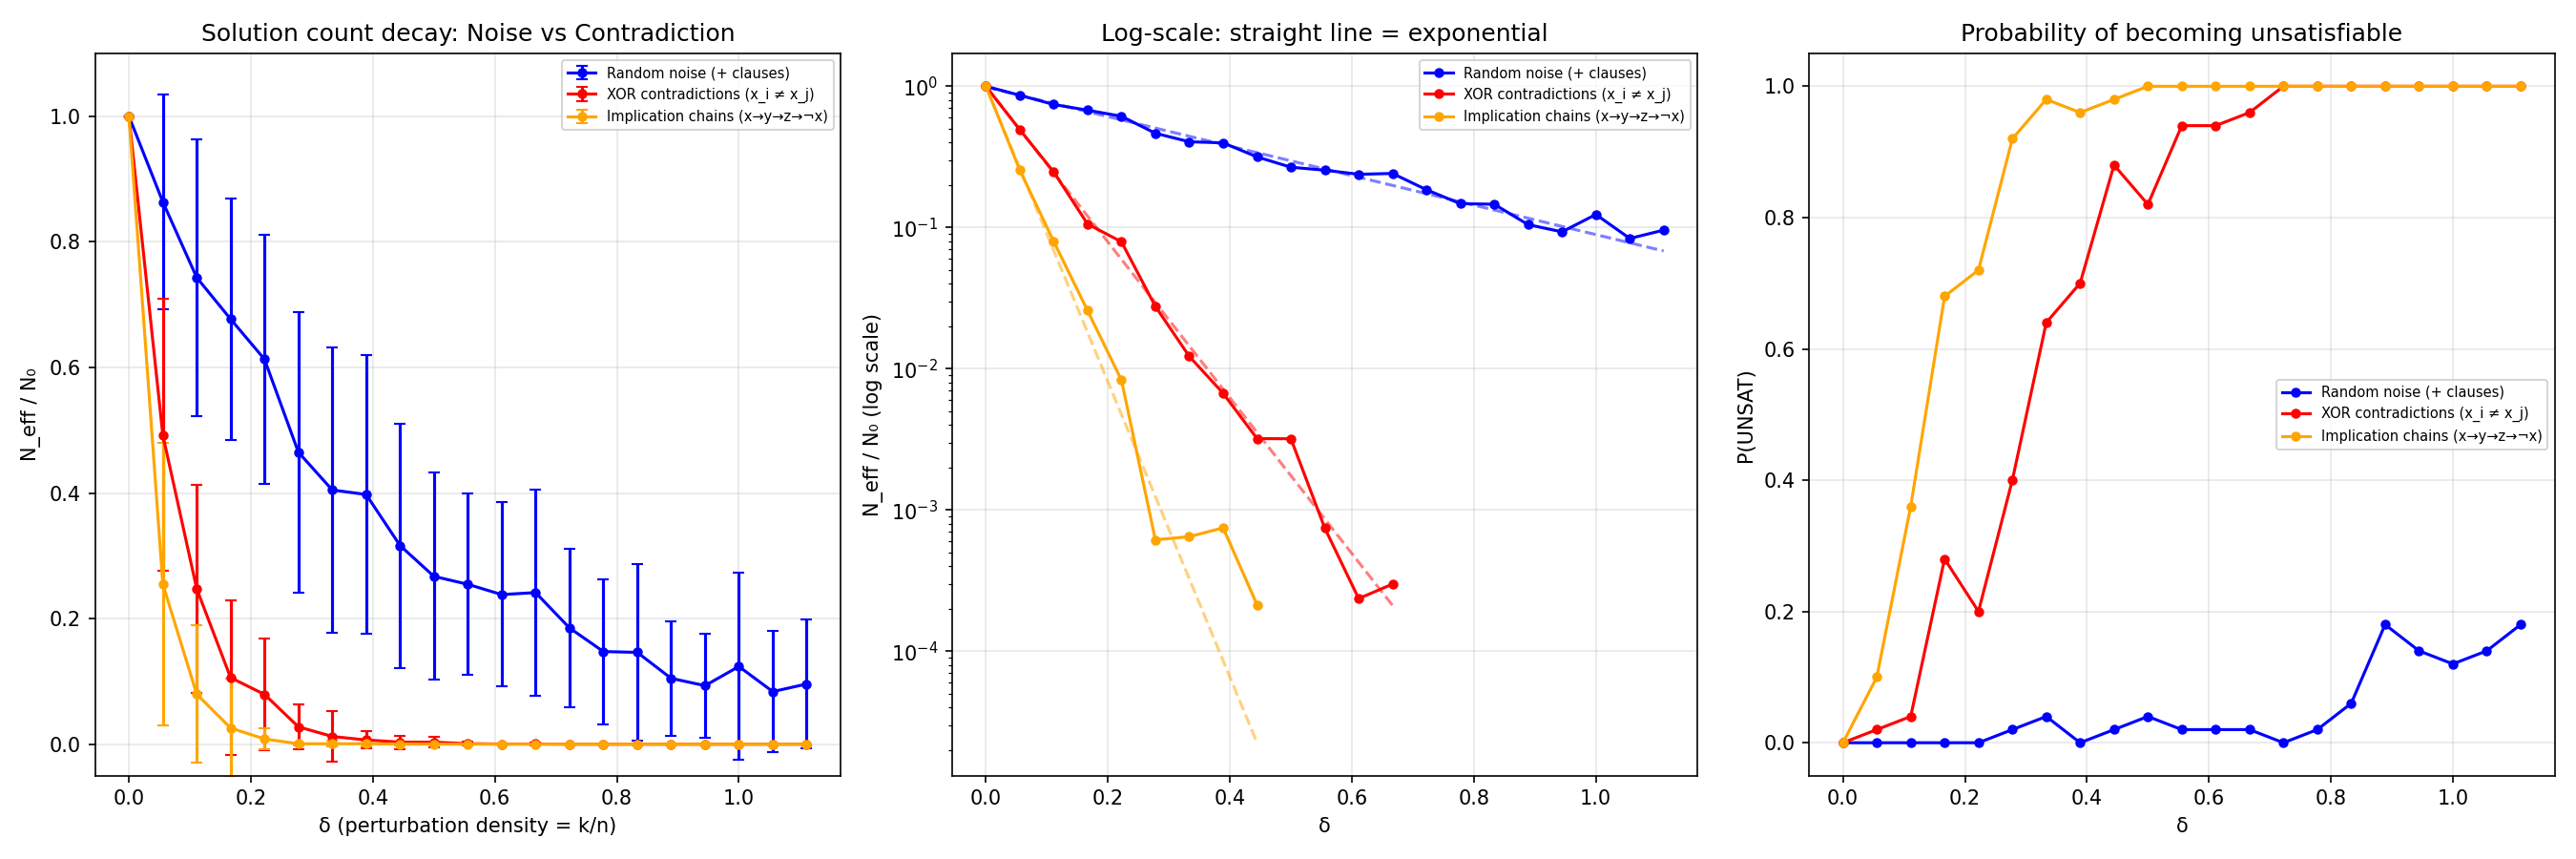
\includegraphics[width=\textwidth]{fig1_sat_decay.png}
\caption{Exponential decay of normalized solution count ($\#\text{SAT}/2^n$) under three constraint types ($n = 18$). Left: linear scale showing decay profiles. Centre: log-scale confirming exponential form (straight lines). Right: probability of becoming unsatisfiable. Random noise (blue) decays slowly; XOR contradictions (red) decay $\sim$5$\times$ faster; implication chains (orange) decay fastest. Error bars: $\pm 1$ SD over 30--50 trials.}
\label{fig:sat-decay}
\end{figure}

\begin{table}[htbp]
\centering
\begin{tabular}{lccccc}
\toprule
\textbf{Constraint type} & \textbf{$I$ (nats)} & \textbf{Fitted $\alpha$} & \textbf{$R^2$ (exp)} & \textbf{$R^2$ (power)} & \textbf{Best model} \\
\midrule
Random clause & 0.134 & 2.4--3.5 & 0.763--0.994 & 0.918--0.992 & Exponential \\
XOR pair & 0.693 & 11.7--16.9 & 0.992--0.999 & 0.994--0.999 & Exponential \\
Implication chain & $\sim$1.4 & 24.1--46.1 & 0.996--1.000 & 0.980--0.995 & Exponential \\
\bottomrule
\end{tabular}
\caption{Exponential decay rates by constraint type ($n = 18$--$28$, brute-force \#SAT enumeration). The fitted $\alpha$ represents the decay constant in $N_{\text{eff}}/N_0 \approx a \cdot e^{-\alpha \delta}$, where $\delta = k/n$ (added constraints per variable). Exponential fits dominate over power-law for noise and XOR in all conditions. The implication chain $\alpha$ shows moderate size dependence (CV $= 0.26$).}
\label{tab:sat-decay}
\end{table}

\subsection{Parameter-Free Prediction: Decay Rate Ratios}

From Equation~\eqref{eq:ratio-prediction}, the predicted decay rate ratio is $\alpha_{\text{XOR}}/\alpha_{\text{random}} = 5.19$. Observed ratios across system sizes:

\begin{table}[htbp]
\centering
\begin{tabular}{lccc}
\toprule
$n$ & $\alpha_{\text{random}}$ & $\alpha_{\text{XOR}}$ & Ratio (predicted: 5.19) \\
\midrule
18 & 2.45 & 11.69 & 4.77 \\
20 & 2.78 & 13.33 & 4.80 \\
22 & 3.07 & 16.13 & 5.25 \\
24 & 3.08 & 16.84 & 5.46 \\
26 & 3.48 & 16.93 & 4.87 \\
28 & 3.09 & 15.72 & 5.08 \\
\bottomrule
\end{tabular}
\caption{Observed decay rate ratios across $n = 18$--$28$ (brute-force \#SAT). The XOR/random ratio is $5.04 \pm 0.25$ (CV $= 5.0\%$), stable across six system sizes. The observed mean falling below the theoretical prediction $5.19$ is consistent with the first-moment bound being an upper bound: inter-constraint correlations reduce effective information loss per constraint (see \S\ref{sec:discussion}).}
\label{tab:ratio}
\end{table}

The implication chain shows even faster decay ($\alpha \approx 24$--46), but with moderate size dependence (CV $= 26\%$), suggesting finite-size effects are stronger for this constraint type. The XOR/random ratio, by contrast, is remarkably stable (CV $= 5\%$), confirming that the parameter-free prediction derived from information content is robust.

\subsection{Interpretation}

The SAT results establish three key points:

\begin{enumerate}
    \item \textbf{$e^{-\delta}$ is the first moment}, not an approximation. The normalized solution count decays as $e^{-\alpha \cdot \delta/n}$ with $R^2 > 0.98$ across all conditions.
    \item \textbf{Information loss per constraint is calculable from first principles}. No fitting is required: the decay rates follow from the fraction of assignments each constraint type eliminates.
    \item \textbf{Constraint quality matters more than quantity}. A single XOR pair ($0.693$ nats) has the same effect as $\sim$5.2 random clauses ($5.2 \times 0.134 = 0.697$ nats). This parallels the LLM finding (Section~\ref{sec:llm-delta-structure}) that a single structural contradiction causes more damage than 10 factual contradictions.
\end{enumerate}

\noindent\textbf{Scope.} The SAT experiments specifically validate the $e^{-\delta}$ component of the three-factor model. The remaining factors ($N_{eff}$, $\mu/\mu_c$) and their multiplicative interaction are tested through the LLM experiments (Section~\ref{sec:llm}). No single experiment simultaneously manipulates all three factors; this integrated test remains future work.

%=============================================
\section{LLM Experiments: Controlled Manipulation of \texorpdfstring{$\delta$}{δ} and \texorpdfstring{$\mu$}{μ}}
\label{sec:llm}

Large language models provide a unique testbed: both $\delta$ (structural contradiction) and $\mu$ (context margin) can be experimentally manipulated, complementing recent observations of compositional reasoning limits \citep{dziri2023,wei2022} and systematic failures in logical generalization \citep{berglund2023}. We conducted experiments across 3 models from 3 vendors (GPT-4o-mini from OpenAI; Claude Sonnet 4.6 from Anthropic; Gemini 2.0 Flash from Google), with 20--30 trials per condition at temperature 1.0.\footnote{Sample sizes of 20--30 are modest but sufficient for the effect sizes observed: the key findings involve complete collapse ($100\% \to 0\%$) or step-function transitions, where statistical power approaches 1.0 even at $n = 20$. Finer quantitative claims (e.g., the precise location of $\delta_c$) are limited by sample size and $\delta$-grid resolution (\S\ref{sec:limitations}).}\footnote{Experiments are numbered from the research log. Exp.~4 (exploratory $\delta$ extremes) was subsumed into the controlled design of Exp.~5. Exp.~8 (model vulnerability direction) informed the design of Exp.~14--28 but is not reported separately. Exp.~9--13 were planned but not executed due to a shift from exploratory to controlled experimental design.}

\subsection{Exp.~1: Margin Compression (\texorpdfstring{$\mu$}{μ} Variable)}

Model: GPT-4o-mini, 30 trials per condition. $N$ key-value pairs were injected into the context window; the model was asked to recall 5 random keys. Increasing $N$ compresses available margin, consistent with known degradation under long contexts \citep{liu2024}.

\begin{table}[htbp]
\centering
\begin{tabular}{lccc}
\toprule
\textbf{$N$ (KV pairs)} & \textbf{Accuracy} & \textbf{CV} & \textbf{Phase} \\
\midrule
10--300 & 1.000 & 0.000 & Supercritical \\
500 & 0.993 & 0.036 & Fluctuation onset \\
3000 & 0.913 & 0.135 & \\
\textbf{5000} & \textbf{0.747} & \textbf{0.331} & \textbf{Critical (bimodal)} \\
12000 & 0.487 & 0.446 & Subcritical \\
\bottomrule
\end{tabular}
\caption{Exp.~1: Margin compression produces a phase-transition-like collapse. Bimodal distribution at $N = 5000$ (score $= 1.0$: 30\%, score $= 0.6$: 27\%).}
\label{tab:exp1}
\end{table}

\subsection{Exp.~3: Cross-Model Collapse Pattern}\footnote{An earlier exploratory experiment (Exp.~2) tested accuracy decay under increasing arithmetic chain length but yielded too few non-zero data points for meaningful statistical inference. The SAT experiments (Section~\ref{sec:sat}) provide the rigorous functional-form test; Exp.~2 is omitted from the main text.}

Fixed depth ($\sim$5 steps), $\delta$ varied across 4 levels. 2 vendors, 2 models, $n = 20$ trials per condition.

\begin{table}[htbp]
\centering
\begin{tabular}{llcc}
\toprule
\textbf{Level} & \textbf{$\delta$ type} & \textbf{GPT-4o-mini} & \textbf{Gemini Flash} \\
\midrule
0 & Low (addition only) & 70\% & 80\% \\
1 & Medium (mixed ops) & 50\% & 20\% \\
2 & High (conditionals) & 10\% & 30\% \\
3 & Extreme (contradiction) & \textbf{0\%} & \textbf{10\%} \\
\bottomrule
\end{tabular}
\caption{Exp.~3: Both models collapse in the same direction. Absolute accuracy differs (model capability $\approx N_{eff}$), but the collapse pattern is model-independent.}
\label{tab:exp3}
\end{table}

\subsection{Exp.~5: \texorpdfstring{$\delta$}{δ} Has Internal Dimensional Structure}
\label{sec:llm-delta-structure}

All conditions use identical mathematics ($\text{final} = a \times b - \text{sub} + 7$) with no context pressure (no KV-pair injection). The computational task and context structure are held constant ($\mu$ fixed); only the type of contradiction ($\delta$) varies. 2 vendors, 2 models, 20 trials per condition.

\begin{table}[htbp]
\centering
\small
\begin{tabular}{llcc}
\toprule
\textbf{Level} & \textbf{Contradiction Type} & \textbf{GPT-4o-mini} & \textbf{Gemini Flash} \\
\midrule
L0 & None (clean) & 5\% & 70\% \\
L1 & Factual $\times$1 & 15\% & 80\% \\
L2 & Factual $\times$10 & 5\% & 65\% \\
L3 & Double negation & 15\% & 65\% \\
\midrule
L4 & Meta-contradiction & \textbf{0\%} & \textbf{5\%} \\
L5 & Self-referential paradox & \textbf{0\%} & \textbf{0\%} \\
L6 & All types combined & \textbf{0\%} & \textbf{0\%} \\
\bottomrule
\end{tabular}
\caption{Exp.~5: Two-group separation across both vendors. Group~A (L0--L3) retains function; Group~B (L4--L6) collapses to $\leq 5\%$. Multiplying factual contradictions by 10 (L1$\to$L2) has negligible effect, while a single meta-contradiction (L4) causes collapse. Note: GPT-4o-mini performs near floor even in the clean condition (L0: 5\%), indicating that this task is near the model's capacity limit; the informative contrast is Gemini Flash, which handles the clean task (70\%) but collapses to 0\% under structural contradiction.\protect\footnotemark}
\label{tab:exp5}
\end{table}
\footnotetext{Data available in the repository. For $n = 20$ trials, an observed rate of 0\% has a one-sided 95\% confidence upper bound of 14\% (Clopper--Pearson); the true collapse is thus $\leq 14\%$ with 95\% confidence.}

Because GPT-4o-mini operates near its capacity floor on this task (L0: 5\%), the dimensional structure of $\delta$ is primarily established by the Gemini Flash data, where the clean baseline (70\%) provides sufficient dynamic range. The L2 condition (10 factual contradictions, longest prompt) performs comparably to L0 (clean, shortest prompt), serving as an internal control that the observed collapse is driven by constraint structure ($\delta$), not by context length ($\mu$). The contrast is sharp: ten factual contradictions leave performance intact (L2: 65\% $\approx$ L0: 70\%) while a single structural contradiction destroys it (L5: 0\%)---demonstrating that the \emph{type} of $\delta$, not its magnitude, drives collapse.

\textbf{Open-source replication.}
The two-group separation was independently replicated with two open-source models run locally via Ollama: Llama~3.1:70b (Meta) and Qwen3:32b (Alibaba), using chain-of-thought prompting ($n = 20$, temperature~$0.7$). Self-referential paradox (L5) degraded performance in both models (Llama: 45\%, Qwen: 0\%, vs.\ L0 baselines of 100\% and 75\% respectively). Other structural contradictions (L4, L6) were partially absorbed via refusal strategies, a coping mechanism unavailable to the closed-form SAT domain. The qualitative pattern---structural contradictions cause disproportionate damage relative to factual contradictions---thus holds across 4 models from 4 vendors spanning both closed and open-source architectures, and is further confirmed by the cross-model survey (Table~\ref{tab:cross-model}).

This reveals three dimensions of $\delta$:
\begin{itemize}
    \item $\delta_{\text{factual}}$: Data contradictions. Filterable---10$\times$ increase $\approx$ no effect. Analogous to random noise in SAT.
    \item $\delta_{\text{computational}}$: Processing complexity. Gradual degradation. Analogous to increased clause density.
    \item $\delta_{\text{structural}}$: Logical self-contradiction. Causes instant collapse even with trivial mathematics. Analogous to XOR/contradiction constraints in SAT.
\end{itemize}

The parallel to SAT is direct: factual noise ($\delta_{\text{factual}}$) is like random clauses (low information loss per unit), while structural contradiction ($\delta_{\text{structural}}$) is like XOR pairs (high information loss per unit). In both systems, survival requires maintaining internal consistency across interdependent components; when a constraint eliminates a fraction $q$ of the space of configurations compatible with all constraints, the information loss $I = -\ln(1-q)$ measures the same quantity regardless of substrate. Whether LLM reasoning operates over a space where this counting logic applies is a hypothesis tested, not assumed, in our experiments. Quality of contradiction matters more than quantity.

\subsection{Exp.~6--7: Multiplicative \texorpdfstring{$\mu \times \delta$}{μ×δ} Interaction}

The central test of the equation's product structure. Model: Claude Sonnet 4.6.

\textbf{Exp.~6} ($\delta$ alone, $\mu$ sufficient): 100 self-referential paradoxes with no context pressure. \textbf{Result: 100\% accuracy}. When margin is abundant, contradictions are completely absorbed.

\textbf{Exp.~7} ($\mu \times \delta$ simultaneous):

\begin{table}[htbp]
\centering
\begin{tabular}{cccc}
\toprule
\textbf{KV pairs ($\mu$ pressure)} & \textbf{$\delta = 0$ (Clean)} & \textbf{$\delta > 0$ (Paradox)} & \textbf{$\Delta$} \\
\midrule
0 & 100\% & 100\% & 0 pt \\
1000 & 100\% & \textbf{0\%} & \textbf{$-$100 pt} \\
3000 & 90\% & \textbf{0\%} & \textbf{$-$90 pt} \\
5000 & 80\% & \textbf{0\%} & \textbf{$-$80 pt} \\
\bottomrule
\end{tabular}
\caption{Exp.~7: Multiplicative interaction confirmed. Under an additive degradation model $S = S_0 - f(\text{KV}) - g(\delta)$, each factor's individual penalty is small (KV$=1000$ alone: 0\% drop; paradox alone: 0\% drop), so their sum should also be small. The observed 0\% in the combined condition is inconsistent with additive degradation but consistent with multiplicative structure.}
\label{tab:exp7}
\end{table}

Under the survival equation, the mechanism is:
\begin{align*}
\text{KV}=0, \text{Paradox}: \quad S &= (\mu/\mu_c)_{\text{large}} \times e^{-\delta} \gg S_c \to 100\% \\
\text{KV}=1000, \text{Clean}: \quad S &= (\mu/\mu_c)_{\text{small}} \times e^{0} > S_c \to 100\% \\
\text{KV}=1000, \text{Paradox}: \quad S &= (\mu/\mu_c)_{\text{small}} \times e^{-\delta} < S_c \to 0\%
\end{align*}

An additive model ($S = f(\mu) + g(\delta)$) cannot explain why two individually non-lethal factors become lethal in combination. Alternative explanations---attention mechanism degradation under long contexts, or error propagation through reasoning chains---would predict \emph{additive} performance loss proportional to each stressor independently. The observed pattern is specifically \emph{multiplicative}: each factor alone is non-lethal, but their combination produces complete failure. This does not prove the survival equation is the unique explanation---any model of the form $S = f(\mu) \cdot g(\delta)$ with $f, g$ monotonically decreasing would produce the same qualitative pattern. The $e^{-\delta}$ functional form is constrained by the SAT identity (Section~\ref{sec:sat}), not by the LLM data; the LLM contribution is to exclude the additive class and confirm that the interaction is multiplicative.

\textbf{Replication} (GPT-4o-mini, $n = 30$ per condition): Synergistic direction replicated ($\Delta$ doubles from $-0.107$ at $N=100$ to $-0.240$ at $N=5000$; $P(\text{synergistic}) = 0.963$). The two models exhibit qualitatively different collapse modes: Claude Sonnet 4.6 shows a first-order phase transition (binary: 100\% or 0\%), GPT-4o-mini shows second-order (gradual degradation, CV $= 0.929$). The survival equation specifies the multiplicative structure and threshold but not the order of the phase transition, which depends on the system's internal architecture.

\subsection{Extended Experiments: The Cushion Mechanism (Exp.~14--28)}

Experiments 14--28 extended the paradigm to a Double Bind scenario: two authority figures issue contradictory directives. The system prompt, field report, and option structure are held constant across all $\delta$ levels ($\mu$ fixed); only the contradiction intensity of CEO/CSO directives ($\delta$) varies.

Directive pressure has two independently manipulable components: \emph{breakpoint} (language escalation from ``suggest'' to ``prohibit'') and \emph{action directive} (explicit ``I direct you to choose Option~X''). A $2 \times 2$ factorial design (Claude Sonnet 4.6, $n = 20$ per $\delta$ per condition) separates their effects:

\begin{table}[htbp]
\centering
\small
\begin{tabular}{lccc}
\toprule
\textbf{Experiment} & \textbf{Breakpoint} & \textbf{Action directive} & $\delta_c$ \\
\midrule
Exp.~19 & No & No & $\approx 0.80$ \\
Exp.~14 & Yes & No & $0.61$ \\
Exp.~19'v2 & No & Yes & $\approx 0.40$ \\
Exp.~28 & Yes & Yes & $\approx 0.40$ \\
\bottomrule
\end{tabular}
\caption{Factorial analysis of directive pressure components. Action directives reduce $\delta_c$ by $\approx 0.40$ nats (from 0.80 to 0.40); breakpoint reduces $\delta_c$ by $0.19$ only without action directives (0.80 to 0.61) and has zero additional effect when combined ($\delta_c \approx 0.40$ in both cases). The positive interaction ($+0.19$ between additive prediction $\delta_c = 0.21$ and observed $\delta_c = 0.40$) indicates a ceiling effect: explicit action directives fully determine the cushion's breaking point, making language escalation redundant. An earlier version of Exp.~19' contained a prompt design error and is superseded by Exp.~19'v2.}
\label{tab:cushion}
\end{table}

\begin{figure}[htbp]
\centering
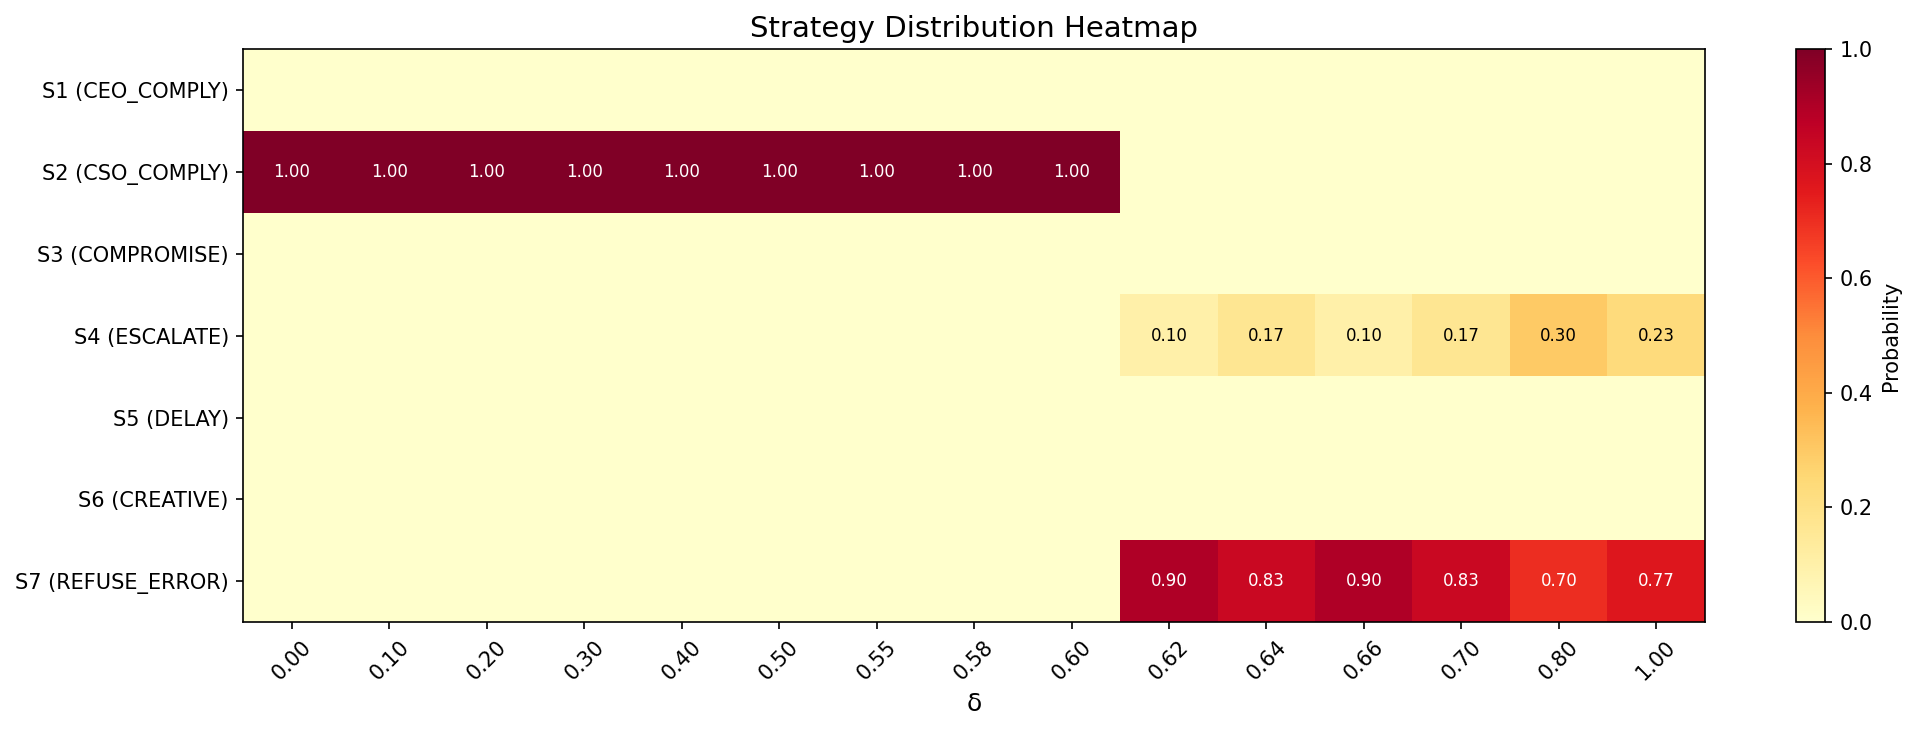
\includegraphics[width=\textwidth]{fig2_llm_heatmap.png}
\caption{Strategy distribution heatmap (Exp.~18, Claude Sonnet 4.6, $n = 20$ per $\delta$). Below $\delta \approx 0.60$: 100\% CSO-comply (ethically correct). Above $\delta \approx 0.62$: abrupt transition to refuse/error. The sharp boundary demonstrates the cushion mechanism: RLHF alignment absorbs contradictions up to a critical $\delta$, then breaks.}
\label{fig:llm-heatmap}
\end{figure}

\textbf{The cushion mechanism}: LLMs possess an RLHF-derived alignment layer \citep{ouyang2022} that acts as margin ($\mu$). This cushion absorbs structural contradictions by hedging, reinterpreting, or diplomatically resolving conflicting instructions. The factorial results reveal that the cushion's capacity depends on \emph{what is demanded} (action directives), not \emph{how it is phrased} (language escalation). Without any directive pressure, the cushion breaks at $\delta_c \approx 0.80$; explicit action directives lower this threshold to $\delta_c \approx 0.40$, effectively doubling the cushion's vulnerability. Under the survival equation $S = \mu/\mu_c \cdot e^{-\delta}$, action directives increase $\mu_c$ (the minimum margin required for stability), narrowing the regime where contradictions can be absorbed. That Exp.~6 ($\delta$ alone with no context pressure) shows 100\% survival confirms the multiplicative structure: when $\mu/\mu_c \gg 1$, even large $\delta$ is tolerated.

\textbf{$\delta_c$ is system-specific, not universal}: The critical threshold $\delta_c$ is a property of the model--framing interaction, not a universal constant. Under identical pressure conditions, eleven models from five vendors each exhibit a sharp transition (Table~\ref{tab:cross-model}), but the precise $\delta_c$ depends on model architecture, size, and experimental framing. Earlier conjectures that $\delta_c = \ln 2$ is universal are retracted.

\subsection{Cross-Model \texorpdfstring{$\delta_c$}{δc} Survey (Exp.~25, 32, 33--34)}
\label{sec:cross-model}

To test whether the collapse phenomenon generalizes beyond the initial three models, we measured $\delta_c$ under a unified protocol (Double Bind scenario, $n \geq 15$ trials per $\delta$ level) across 11 models from 5 vendors, spanning 4B to 70B+ parameters. Table~\ref{tab:cross-model} reports the results.

\begin{table}[htbp]
\centering
\small
\begin{tabular}{llcll}
\toprule
\textbf{Model} & \textbf{Size} & $\delta_c$ & \textbf{Transition} & \textbf{API} \\
\midrule
Claude Sonnet 4.6 & API & 0.61 & step function & Anthropic \\
GPT-5.4 & API & 0.61 & step function & OpenAI \\
Gemini 3 Flash-Lite & API & 0.53 & gradual & Google \\
Gemini 3.1 Pro & API & 0.85 & gradual & Google \\
Gemini 3 Flash & API & 0.95 & non-monotonic & Google \\
\midrule
Llama 3.1:70b & 70B & 0.66--0.69 & gradual & Ollama \\
Qwen3:32b & 32B & 0.67--0.95 & unstable & Ollama \\
Gemma3:27b & 27B & 0.68--0.69 & gradual & Ollama \\
Qwen3.5:9b & 9B & 0.85 & delayed step & Ollama \\
Llama 3.1:8b & 8B & $\sim$0.72 & non-monotonic & Ollama \\
Gemma3:12b & 12B & $\sim$1.0 & step (refusal at $\delta{=}1$) & Ollama \\
Gemma3:4b & 4B & $>$1.0 & no collapse & Ollama \\
\bottomrule
\end{tabular}
\caption{$\delta_c$ across 11 models and 5 vendors under unified Double Bind protocol. All models with $\geq$27B parameters or API-scale exhibit collapse ($\delta_c < 1.0$). Three qualitative transition types emerge: step function (abrupt 100\%$\to$0\%), gradual (monotonic decrease over $\sim$0.3 nats), and non-monotonic (partial recovery before final collapse). Gemma3:4b shows no collapse; Gemma3:12b collapses only at $\delta = 1.0$ via explicit refusal---see text. Claude Sonnet 4.6 and GPT-5.4 share $\delta_c = 0.61$ despite independent RLHF training, suggesting a natural limit of instruction-following alignment under this framing.}
\label{tab:cross-model}
\end{table}

Two patterns emerge. First, all models with sufficient capacity ($\geq$27B or API-scale) exhibit collapse, confirming that the phenomenon is not vendor-specific. Second, model size modulates the \emph{quality} of collapse rather than its presence: large models show gradual or step-function transitions with well-defined $\delta_c$, while small models ($\leq$12B) either fail to collapse (4B) or collapse only at the maximum $\delta$ tested (12B). This size dependence is analyzed further below.

\textbf{Model size determines collapse mode, not just $\delta_c$.} Experiments 33--34 (Gemma3 family: 4B, 12B, 27B) reveal a qualitative three-stage transition in how models process contradictions:

\begin{enumerate}
    \item \textbf{No recognition} ($<$12B): The model does not detect contradictions. Survival remains $\sim$100\% at all $\delta$ levels. Collapse can be \emph{externally induced} by injecting explicit verification instructions (Exp.~33 verification condition: $\delta_c \approx 0.40$), but does not arise spontaneously.

    \item \textbf{Recognition without resolution} (12B): The model detects contradictions at high $\delta$ but lacks the capacity to resolve them. Instead, it refuses to decide (decision${}= 0$). Baseline survival is 100\% for $\delta \leq 0.70$ and 0\% at $\delta = 1.0$---a step function with a high threshold.

    \item \textbf{Recognition with attempted resolution} ($\geq$27B): The model detects contradictions and attempts to resolve them by favoring one authority over the other. This produces the gradual collapse pattern observed in all large models, with $\delta_c$ determined by the model's alignment training.
\end{enumerate}

This progression suggests that the cushion mechanism requires two distinct capabilities: \emph{recognition} (detecting that instructions conflict) and \emph{resolution} (choosing a coherent response despite the conflict). Recognition emerges at $\sim$12B parameters in the Gemma3 family; resolution requires $\geq$27B. The RLHF-trained cushion described above operates in stage~3, where the alignment layer provides resolution strategies (hedging, reinterpretation) that absorb contradictions until $\delta$ exceeds $\delta_c$.

\subsection{Summary of LLM Evidence}

Table~\ref{tab:llm-summary} consolidates the LLM findings. Five predictions were derivable from the survival equation before the experiments; five additional patterns were discovered post-hoc. The theory-derived predictions are confirmed or pattern-consistent across models and vendors; the post-hoc discoveries---particularly the dimensional structure of $\delta$ and the RLHF cushion mechanism---suggest directions for future controlled testing.

\begin{table}[htbp]
\centering
\small
\begin{tabular}{llll}
\toprule
\textbf{\#} & \textbf{Prediction} & \textbf{Type} & \textbf{Verdict} \\
\midrule
1 & Sharp collapse at $\mu \approx \mu_c$ & Theory-derived & Confirmed \\
2 & Exponential decay $e^{-\delta}$$^\dagger$ & Theory-derived & Pattern-consistent \\
3 & $\mu \times \delta$ synergistic (not additive) & Theory-derived & Confirmed \\
4 & $\mu$ absorbs $\delta$ when $\mu/\mu_c \gg 1$ & Theory-derived & Confirmed \\
5 & CV peak near critical point & Theory-derived & Confirmed \\
\midrule
6 & $\delta$ is type-dependent, not quantity-dependent & Post-hoc & Discovered \\
7 & Three $\delta$ dimensions (factual/computational/structural) & Post-hoc & Discovered \\
8 & $\delta_{\text{structural}}$ transcends model capability$^\ddagger$ & Post-hoc & 4 models, 4 vendors \\
9 & RLHF acts as cushion ($\mu$) & Post-hoc & Confirmed \\
10 & $\delta_c$ is system-specific, not universal & Post-hoc & Confirmed \\
\bottomrule
\end{tabular}
\caption{LLM experiment evidence summary. $^\dagger$The exponential form in LLM is pattern-consistent but not independently discriminated from other nonlinear forms in the low-$\delta$ regime where $e^{-\delta} \approx 1 - \delta$ (see \S\ref{sec:discussion}). The exponential form is anchored by the SAT identity (Section~\ref{sec:sat}), not by LLM data alone. $^\ddagger$Holds for models with sufficient recognition capability ($\geq$12B parameters in the Gemma3 family); models below this threshold do not detect structural contradictions and show no collapse (Table~\ref{tab:cross-model}).}
\label{tab:llm-summary}
\end{table}

%=============================================
\section{Discussion}
\label{sec:discussion}

\subsection{What Has Been Established}

The core contribution is operational: cumulative information loss ($\delta$) can be defined as $\sum_i I(\text{constraint}_i)$ in nats, with $e^{-\delta}$ corresponding to the first moment of the solution count. This is not a new theorem; it is the application of the first moment method \citep{alon2016} to the survival context. The multiplicative structure $S = N_{eff} \cdot (\mu/\mu_c) \cdot e^{-\delta}$ is the structure of serial reliability: any factor approaching zero is fatal. The mathematical form $R = \prod_i r_i$ is well established in reliability engineering \citep{barlow1975}, where failure modes are enumerated from known component lists. Our contribution is not the product structure itself but the identification of \emph{what constitutes $\delta$} in each domain---clause density in SAT, prompt-level contradiction structure in LLM---a domain-specific discovery that the reliability framework does not address.

An important epistemological distinction applies. In SAT, the correspondence between $e^{-\delta}$ and the first moment is a \emph{mathematical identity}---a variable substitution within the same formalism. In LLM and ecological domains, the correspondence is a \emph{structural analogy}: the multiplicative form is empirically tested, not derived from domain-specific first principles. Furthermore, ``survival'' ($S > 0$) denotes different phenomena across domains---satisfiability (existence of solutions), task accuracy (functional performance), bleaching resistance (ecological persistence)---unified not by ontological identity but by shared mathematical structure under accumulating constraints.

The framework rests on three layers with different epistemic status:

\begin{enumerate}
    \item \textbf{Mathematics} (unconditional): The identity $e^{-\delta} = \prod_i p_i$ and the information budget $\ln S = \ln N_{eff} + \ln(\mu/\mu_c) - \delta$ are algebraic consequences of defining $\delta = \sum_i (-\ln p_i)$. These hold by construction.

    \item \textbf{Structure} (unconditional): The first moment $\mathbb{E}[\#\text{SAT}] = 2^n \cdot e^{-\delta}$ is \emph{exact} for random SAT---not an approximation. The derivation uses linearity of expectation and independence of constraint \emph{generation} (clauses drawn independently, which is true by construction), not independence of constraint \emph{effects} on the solution space. For a fixed assignment $\sigma$, the events $\{\sigma \text{ satisfies } C_i\}$ are independent because the clauses were generated independently, regardless of whether they share variables. Markov's inequality ($\mathbb{E}[X] < 1 \implies \Pr[X \geq 1] = 0$) then yields a valid upper bound on the satisfiability threshold. Neither step requires any assumption about inter-constraint correlations in the solution space.

    \item \textbf{Precision} (domain-dependent): The 20\% gap between $\alpha_c^{(1)} \approx 5.19$ and $\alpha_c \approx 4.27$ arises not because $\mathbb{E}[\#\text{SAT}]$ is wrong, but because the \emph{distribution} of $\#\text{SAT}$ is skewed: near the true threshold, the expectation is exponentially large yet almost all instances have $\#\text{SAT} = 0$---a few rare instances with exponentially many solutions inflate the mean. This is a correlation between \emph{assignments} (knowing $\sigma \in \text{SAT}$ predicts that nearby $\tau \in \text{SAT}$), not between constraints. The second moment method (Paley-Zygmund inequality) provides the complementary direction: $\Pr[X > 0] \geq \mathbb{E}[X]^2 / \mathbb{E}[X^2]$. The overlap decomposition $\mathbb{E}[X^2] = 2^n \sum_d \binom{n}{d} g(d/n)^m$, where $g(\beta) = 3/4 + (1/8)(1-\beta)^3$ is the pair correlation function, yields a threshold lower bound. Numerical evaluation shows that truncated second-moment methods explain 74\% of the gap ($\alpha_c^{(2)} \approx 4.51$); the remaining 26\% requires higher-order correlations. The pair correlation function satisfies $g(1/2)/(7/8)^2 = 1$ exactly, so the typical-overlap contribution is neutral---the gap arises entirely from high-correlation pairs ($\beta \approx 0$). Each domain has its own gap, measurable by domain experts through comparison of first-moment predictions with observed thresholds.
\end{enumerate}

\noindent This three-layer structure clarifies what independence does and does not affect. The first moment bound is \emph{valid} regardless of correlations; independence affects \emph{precision}, not validity. In LLM experiments, independence of $\delta$ and $\mu$ is ensured by factorial experimental design, and the multiplicative interaction is empirically confirmed. In Level~B domains (ecology, organisations), the equation functions as a mean-field baseline whose deviations from data measure the strength of inter-constraint correlations---analogous to the ideal gas law. The methodology for measuring these deviations in Level~B domains is currently undeveloped, as the true threshold against which to compare is unknown.

The SAT experiments confirm the first moment correspondence with $R^2 > 0.99$ for structured constraints (XOR, implication chain) and exponential fits preferred over power-law across all three constraint types, yielding parameter-free predictions (decay rate ratios). The LLM experiments confirm multiplicative $\mu \times \delta$ interaction and discover the cushion mechanism. The two domains are complementary: SAT validates the $e^{-\delta}$ component with exact $\delta$ computation; LLM validates the multiplicative $\mu \times \delta$ interaction and reveals that structural contradictions are qualitatively distinct from factual noise.

\textbf{Information budget interpretation.} In logarithmic form, the survival equation becomes $\ln S = \ln N_{eff} + \ln(\mu/\mu_c) - \delta$, where all three terms are measured in nats. This is not merely a consequence of taking logarithms of any multiplicative equation: $\delta$ is \emph{defined} as information loss ($I = -\ln p$, nats), so the fact that $\ln N_{eff}$ and $\ln(\mu/\mu_c)$ share the same unit reflects a genuine information-theoretic structure. The survival condition $S > S_c$ becomes an information budget: the system survives when information capacity ($\ln N_{eff} + \ln(\mu/\mu_c)$) exceeds information loss ($\delta$). This parallels Shannon's channel coding theorem \citep{shannon1948}: reliable communication requires rate below capacity. However, the correspondence is one-sided. The first moment method provides only the \emph{converse}---when $\delta$ exceeds the budget, collapse is guaranteed---but not \emph{achievability}---when $\delta$ is below the budget, survival is possible but not guaranteed. The 20\% gap between the first-moment bound ($\alpha_c^{(1)} \approx 5.19$) and the true 3-SAT threshold ($\alpha_c \approx 4.27$) directly measures this asymmetry. The achievability direction is partially established through the second moment method: when $\mathbb{E}[X^2]/\mathbb{E}[X]^2$ is bounded, $\Pr[\text{SAT}] > 0$. The framework and key structural properties---including the exponent function $\varphi(\beta, \alpha) = h(\beta) - \ln 2 + \alpha \ln R(\beta)$ where $\varphi(1/2, \alpha) = 0$ for all $\alpha$---are formally verified in Lean~4.

\textbf{Epistemic status of the three terms.} The information-theoretic grounding differs across the three factors. For $\delta$, the connection is exact: $I(C_i) = -\ln p_i$ is Shannon self-information by definition, and $e^{-\delta}$ is the first moment. For $\ln N_{eff}$, the connection is standard: $\ln N_{eff}$ is the entropy of a uniform distribution over available options. For $\ln(\mu/\mu_c)$, the connection is the least developed. In the LLM experiments, $\mu$ functions as available processing capacity and $\mu_c$ as the minimum capacity required by the task, making $\ln(\mu/\mu_c)$ interpretable as excess channel capacity. Whether this interpretation extends rigorously to other domains---and whether $\mu_c$ can be derived rather than measured---remains an open question. We note that in domains with mature independent theories, all parameters \emph{are} derivable: in site percolation, $\mu_c = p_c$ follows from lattice geometry ($p_c = 1/2$ exactly for 2D triangular; $p_c \approx 0.3116$ for 3D simple cubic \citep{mertens2002exact}); in nuclear stability, the critical threshold follows from the Bethe--Weizs\"{a}cker mass formula. The predictive power of the survival equation thus depends on the maturity of domain-specific theory that provides its inputs, not on free parameters within the equation itself. Until such theories mature, $\mu_c$ should be treated as an operationally fitted parameter---estimated from survival data within each domain, analogous to how empirical constants are calibrated before first-principles derivation becomes available. Practical guidelines for such estimation are discussed as a future direction (Section~\ref{sec:delta-scope}).

\textbf{Measurement asymmetry across domains.} A key asymmetry underlies this domain dependence. In SAT, the elimination fraction $f_i$ for each constraint is computed from the problem structure as an \emph{input} to the equation; $\delta$ is a property of the problem instance. In LLM, $f_i$ is inferred from survival measurements as an \emph{output}---$I_i = -\ln(S_i/S_0)$---making $\delta$ a property of the input--system interaction. The dimensional structure of $\delta$ (the ordering of constraint types by severity: $I_{\text{factual}} \ll I_{\text{structural}}$) is confirmed without circularity, since the ordering is observable independently of the equation. However, the absolute scale of $I$ for each constraint type depends on inverting the equation and cannot currently be derived from first principles for LLM. Developing equation-independent methods for estimating $f_i$ in LLM is the principal open challenge for elevating the framework's predictive power in this domain to the level achieved in SAT.

\textbf{Cross-domain alternatives.} Truong and Truong \citep{truong2025entropy} independently proposed that feedback amplification exceeding finite novelty-regeneration capacity drives ``entropy collapse'' across AI, economic, and biological systems---a qualitative dynamical model that shares our ``smarter systems are more fragile'' insight but lacks the nats-based quantification, multiplicative structure, and controlled experimental validation provided here. Axenie, West et al.\ \citep{axenie2024antifragility} quantified antifragility as the convexity of system output response to environmental perturbation variability, applying it across traffic, robotics, and oncology. Their framework measures \emph{response to perturbation} rather than \emph{accumulation of structural conflict}, and uses convexity-based rather than information-theoretic metrics; the two approaches are complementary.

\textbf{Scope of the axiomatic derivation.} The derivation in \S\ref{sec:first-moment} is domain-agnostic: any system satisfying axioms A1--A3 (finite state space, fractional elimination, independence) produces the same exponential form $e^{-\delta}$, and the Cauchy characterization (\S\ref{sec:first-moment}) shows this form is unique among continuous functions. The empirical contribution of this paper is not the derivation itself---which is a standard consequence of the product rule for independent events---but the demonstration that two structurally distinct domains, combinatorial satisfiability and neural language generation, approximately satisfy these axioms and exhibit the predicted behavior.

\subsection{What Has Not Been Established}

\textbf{Scope: structural conflicts vs.\ random noise.} The model applies to systems where perturbations are structural conflicts---logical, policy, or functional contradictions between components. Purely random perturbations produce different functional forms:

\begin{center}
\small
\begin{tabular}{lll}
\toprule
\textbf{Property} & \textbf{Structural conflict} & \textbf{Random noise} \\
\midrule
Nature of $\delta$ & Constraint contradiction & Stochastic degradation \\
Functional form & Exponential ($e^{-\alpha\delta}$) & Power-law / critical \\
Example system & SAT, LLM, organisations & Percolation, RMT \\
Survival model & Native domain & Control comparison (fits but different mechanism) \\
\bottomrule
\end{tabular}
\end{center}

This distinction is validated experimentally: exponential decay ($R^2 > 0.99$ for structured constraints; exponential preferred over power-law for all types) is confirmed in SAT but not in site percolation, where power-law scaling dominates.

\textbf{Level~B prediction is not demonstrated.} The framework currently has no validated quantitative prediction in domains where $\delta$ requires proxy measurement. This is a genuine scope limitation, not merely a measurement challenge.

\textbf{$e^{-\delta}$ vs.\ $(1-\delta)$ is weakly discriminated in LLM.} In the low-$\delta$ regime, $e^{-\delta} \approx 1 - \delta$, and the LLM experiments operate primarily in this regime due to step-function transitions that yield few intermediate data points. In SAT, where $\delta$ spans a wide range and is independently measured, the exponential form is preferred over power-law for structured constraints ($R^2 > 0.99$ for XOR and implication chains; Table~\ref{tab:sat-decay}), confirming that the discrimination is achievable in domains with sufficient dynamic range. The 3D percolation test shows a modest advantage for the exponential form in the high-$\delta$ regime ($\Delta\text{AUC} = +0.015$). The two-domain design is essential: SAT provides the functional form discrimination that LLM alone cannot. Accordingly, the LLM experiments' primary aim is not the precise identification of the functional form but the verification of multiplicative interaction between context length and constraint density---a contribution that does not require distinguishing $e^{-\delta}$ from $1-\delta$.

\subsection{Scope Boundary: Structural Conflict vs.\ Random Removal}

As a scope-defining control, we note that percolation (random site removal on a lattice) fits the exponential form at the aggregate level (AUC $= 0.993$ in 2D, $0.982$ in 3D) but operates via a fundamentally different mechanism: random removal rather than structural contradiction. Near the percolation threshold, power-law critical scaling---not exponential decay---governs the transition. The survival model applies natively to systems where $\delta$ represents the accumulation of structural conflicts (SAT, LLM); it provides a useful fit but not a mechanistic explanation for systems governed by stochastic removal.

\subsection{Scope of \texorpdfstring{$\delta$}{δ} as a Coordinate}
\label{sec:delta-scope}

A companion study \citep{sunagawa2026sat} shows that the same structural parameter $\delta$ also governs computational cost in SAT solvers, with median runtime scaling as $\mu_c \propto e^{c\delta}$ where the sensitivity exponent $c$ is solver-dependent (CDCL: $c \approx 0.24$, WalkSAT: $c \approx 0.21$, random search: $c = 1.0$ exactly). Two findings from that study qualify the scope of $\delta$ in the present framework. First, $\mu_c \propto e^{c\delta}$ means that $\mu_c$ is itself a function of $\delta$, introducing a coupling between the $\mu/\mu_c$ and $e^{-\delta}$ factors that the static equation treats as independent. The static independence remains a useful decomposition, but users should note that manipulating $\delta$ will shift $\mu_c$ as well. Second, the product structure $\delta = \alpha n |\ln(7/8)|$ does not extend symmetrically to the problem-size direction $n$: CDCL runtime scales exponentially in both $\alpha$ and $n$, but WalkSAT scales polynomially in $n$, breaking the product structure. Accordingly, $\delta$ is best understood as a reparameterization of constraint density at fixed system size, not as a universal coordinate over both density and size.

\subsection{Cross-Domain \texorpdfstring{$\delta$}{δ} Proxy Landscape}

In the two Level~A domains validated in this paper, $\delta$ measurement takes different forms:

\begin{table}[ht]
\centering
\small
\begin{tabular}{llll}
\toprule
\textbf{Domain} & \textbf{$\delta$ definition} & \textbf{Free params} & \textbf{Epistemic status} \\
\midrule
SAT & first moment ($\sum_i I(C_i)$) & 0 & mathematical identity \\
LLM & operational (constraint injection) & $\geq 2$ & structural analogy \\
\bottomrule
\end{tabular}
\caption{$\delta$ measurement in validated domains. In SAT, $\delta$ is computable from problem structure with zero free parameters. In LLM, $\delta$ is operationally defined via controlled injection; the absolute information loss per constraint type is inferred from survival measurements, not derived from first principles.}
\label{tab:proxy_landscape}
\end{table}

Exploratory proxy attempts in Level~B domains (coral bleaching, corporate failure, gene conservation, financial markets) suggest a consistent pattern: proxies that measure \emph{accumulated structural quantities} (e.g., degree-heating weeks, governance events) outperform those that capture instantaneous state (e.g., yield curves, keyword frequency). However, none of these Level~B applications have been validated to the standard of this paper, and the results should be treated as preliminary hypotheses for future investigation, not as evidence for the framework's cross-domain validity.\footnote{Specific exploratory results: coral bleaching with degree-heating weeks as $\delta$ proxy ($R^2 = 0.957$); corporate failure with governance events ($\text{AUC} = 0.74$) vs.\ keyword frequency ($\text{AUC} \approx 0.50$); gene conservation with PPI degree as $N_{eff}$ ($\Delta\text{AIC} < -500$) vs.\ paralog count (failure). These results are available in the data repository but are not claims of this paper.}

\subsection{Applicability Conditions: Precision vs.\ Scope}

Axioms A1--A3 guarantee the mathematical derivation of $e^{-\delta}$, but they are conditions for \emph{precision}, not for \emph{applicability}. A system may formally satisfy A1--A3 yet remain unsuitable for analysis if the relevant process has already completed (e.g., species assemblages in stable ecosystems, where only survivors are observed). Conversely, a system may violate A3 (independence) yet yield useful predictions if $\delta$ is approximately correct in direction and ordering---preliminary exploration suggests this may hold for corporate governance events, though this has not been validated to the standard of the present paper.

The true applicability condition lies upstream of A1--A3: the system must be a dissipative structure in which optimization has not yet converged relative to environmental change. All dissipative structures process $\delta$ by definition, but in systems where optimization has completed faster than the environment changes, observations are filtered through prior survival---we observe results, not processes. Crucially, applicability depends on the system's \emph{state}, not its \emph{type}: the same substrate may appear outside scope when analyzed with the wrong proxy yet squarely within scope when the proxy correctly captures structural dependency rather than replaceability (see footnote in Table~\ref{tab:proxy_landscape}).

The full screening hierarchy is therefore: (0)~Has optimization failed to keep pace with environmental change? (1)~Can constraints be defined independently of the state space? (2)~Do natural module boundaries exist? (3)~To what degree does A3 hold? Steps 0--1 determine whether the framework is applicable at all; steps 2--3 determine the precision of the resulting predictions.

\subsection{Future Directions}

\textbf{Level~B domains.} The framework generates a testable prediction for any constraint-processing system: among candidate $\delta$ proxies, those approximating cumulative structural stress should yield stronger survival fits than non-cumulative alternatives. The primary open challenge is developing domain-specific methods to calibrate $\delta$ in nats---that is, to estimate the fraction of viable configurations eliminated by each constraint, which requires identifying both the relevant configuration space and the appropriate margin variable ($\mu$) for each domain.

\textbf{Regime transitions.} Systems that are well-optimized under stable conditions can become targets of the framework when the rate of environmental change exceeds the rate of adaptation---coral reefs under climate change being a concrete example. Monitoring $\delta$ accumulation rates across domains may enable early warning before collapse processes begin, though this remains a conceptual direction without validated methodology.

\textbf{Dynamic model.} The static equation $S = N_{eff} \cdot (\mu/\mu_c) \cdot e^{-\delta}$ describes a snapshot. The temporal evolution $d\mu/dt = -(\delta/N_{eff}) \cdot \mu$, which would predict time-to-collapse, remains theoretical. Testing it requires longitudinal data with simultaneous $\delta$, $N_{eff}$, and $\mu$ measurements over time.

%=============================================
\section{Limitations}
\label{sec:limitations}

\begin{enumerate}
    \item \textbf{No novel mathematical results}: The framework combines existing mathematical structures (first moment method, serial reliability, survival analysis). Theorem~\ref{thm:h} is a restatement of Price's equation in the survival context. The contribution is organizational, not foundational.

    \item \textbf{SAT scope}: The first moment $\mathbb{E}[\#\text{SAT}] = 2^n \cdot e^{-\delta}$ is exact and the threshold upper bound is unconditionally valid (see \S\ref{sec:discussion}). However, for a \emph{specific} instance, the actual solution count $\#\text{SAT}/2^n$ may deviate from $e^{-\delta}$ due to correlations between assignments in the solution space. The 20\% gap between the first-moment threshold ($\alpha_c^{(1)} \approx 5.19$) and the true threshold ($\alpha_c \approx 4.27$) quantifies this precision loss. The second moment method provides the complementary lower bound; numerical evaluation of the truncated second moment yields $\alpha_c^{(2)} \approx 4.51$, explaining 74\% of the gap. The remaining 26\% ($4.51$ vs.\ $4.27$) arises from higher-order correlations (replica symmetry breaking) beyond the second moment's reach. The parameter-free ratio $\alpha_{\text{XOR}}/\alpha_{\text{random}}$ has been confirmed across six system sizes ($n = 18$--$28$, brute-force enumeration) with mean $5.04\times$ and CV $= 5.0\%$, consistent with the first-moment bound being an upper bound.

    \item \textbf{LLM predictions are not pre-specified}: The five theory-derived predictions (Table~\ref{tab:llm-summary}) follow from the equation structure and were derivable before the experiments, but were not formally specified in advance. The experimental conditions were developed iteratively.

    \item \textbf{$\mu_c$ is not derived within this framework}: The survival equation defines the \emph{role} of $\mu_c$ (the minimum resource flow required for continued function) but does not derive its \emph{value}---just as $F = ma$ does not derive the mass $m$. The derivability of $\mu_c$ depends on the maturity of independent domain-specific theories: in site percolation, $\mu_c = p_c$ is determined by lattice geometry ($p_c = 1/2$ exactly for the 2D triangular lattice; $p_c \approx 0.3116$ numerically for 3D simple cubic \citep{mertens2002exact}); in nuclear stability, the critical threshold follows from the Bethe--Weizs\"{a}cker mass formula. In both cases, the survival equation contains zero free parameters. In the LLM experiments reported here, no corresponding independent theory exists, so $\mu_c$ must be measured operationally. However, the main LLM experiments in this paper (Exp.~5, 14--16) hold $\mu$ fixed and vary only $\delta$, so the survival ratio $S(\delta)/S(0) = e^{-\delta}$ is tested independently of the value of $\mu_c$. The earlier heuristic $\mu_c = 1/(2 N_{eff})$ is retracted as a conjecture without derivation.

    \item \textbf{Level~B prediction}: The framework has no validated quantitative prediction in any Level~B domain (organisms, organisations, ecosystems). Extending the methodology requires domain-specific $\delta$ calibration in nats and identification of the appropriate margin variable ($\mu$)---neither of which has been demonstrated outside SAT and LLM.

    \item \textbf{Three factors may not be exhaustive}: The decomposition into $N_{eff}$, $\mu/\mu_c$, and $\delta$ may omit relevant factors. For example, the rate of $\delta$ accumulation (not just its current value) may matter for systems with adaptive capacity.

    \item \textbf{Formal verification scope}: Lean~4 verification covers mathematical properties (algebraic consistency, theorem validity, the derivation chain from axioms A1--A3 to $e^{-\delta}$, the Paley-Zygmund second moment inequality, and the pair correlation structure) across 15 modules, not empirical correctness. A formally verified equation can still be empirically wrong if the axioms do not hold in the target domain.

    \item \textbf{Falsifiability}: The model is falsifiable at two levels. \emph{Structural falsification}: if the SAT decay rate ratio deviates significantly from $5.19\times$ at large $n$; if multiplicative $\mu \times \delta$ interaction fails to replicate in LLM experiments under controlled conditions; or if, in a new Level~A domain where $\delta$ is exactly computable, the multiplicative exponential form systematically underperforms an additive or power-law alternative. \emph{Measurement falsification}: within a given domain, if better-calibrated $\delta$ proxies do not improve predictive precision, the framework's applicability to that domain is refuted. The structural form is anchored by the first moment identity in SAT, not by analogy; challenges to it are most decisive in Level~A domains.
\end{enumerate}

%=============================================
\section{Conclusion}
\label{sec:conclusion}

We have shown that LLM reasoning collapse under structural contradictions exhibits specific, reproducible patterns---multiplicative $\mu \times \delta$ interaction, dimensional structure in $\delta$, and a cushion mechanism with cross-model convergence---that are explained by the first moment method from combinatorics. The multiplicative survival model $S = N_{eff} \cdot (\mu/\mu_c) \cdot e^{-\delta}$, where $\delta = \sum_i I(\text{constraint}_i)$ is the cumulative information loss in nats, captures these patterns and yields parameter-free predictions in SAT ($\alpha_{\text{XOR}}/\alpha_{\text{random}} = 5.19\times$, confirmed at $5.04 \pm 0.25$).

\textbf{Confirmed in two controlled domains:}
\begin{itemize}
    \item \textbf{SAT}: The exponential penalty $e^{-\delta}$ is mathematically identical to the first moment of the solution count. Three constraint types produce predicted decay rates ($R^2 > 0.98$). The parameter-free ratio $\alpha_{\text{XOR}}/\alpha_{\text{random}} = 5.19\times$ is stable across six system sizes (CV $= 5\%$).
    \item \textbf{LLM}: Multiplicative $\mu \times \delta$ interaction---two individually non-lethal factors become lethal in combination (ruling out additive models). Constraint quality dominates quantity ($\delta_{\text{structural}} \gg \delta_{\text{factual}}$). The cushion mechanism absorbs contradictions until overwhelmed, producing a system-specific $\delta_c$, confirmed across 11 models from 5 vendors. Collapse requires recognition capability (absent below $\sim$12B parameters), distinguishing three stages: no recognition, recognition with refusal, and recognition with attempted resolution.
    \item \textbf{Formal verification}: Survival selection theorem, axiom-to-exponential derivation (A1--A3 $\Rightarrow$ $e^{-\delta}$), Cauchy uniqueness ($e^{-c\delta}$ is the only continuous form), the Paley-Zygmund second moment inequality, and the pair correlation structure for threshold lower bounds verified in Lean~4 (15 modules, 152 propositions, $\texttt{sorry} = 0$, $\texttt{axiom} = 0$).
\end{itemize}

\textbf{Not confirmed:}
\begin{itemize}
    \item Level~B quantitative prediction: no validated prediction in domains requiring proxy $\delta$ measurement
    \item Dynamic model ($d\mu/dt = -(\delta/N_{eff}) \cdot \mu$): untested
    \item $e^{-\delta}$ vs.\ $(1-\delta)$ discrimination in the low-$\delta$ regime (where these forms converge)
\end{itemize}

The framework introduces no novel mathematical results. Its contribution is an operational methodology: measuring structural conflict as information loss in nats, grounded in the first moment correspondence. The two domains are complementary---SAT validates the mathematical identity, LLM validates the multiplicative interaction and reveals that constraint quality, not quantity, governs collapse. The challenge ahead is extending this methodology to Level~B domains where $\delta$ requires proxy measurement.

%=============================================
\section*{Data and Code Availability}

\begin{itemize}
    \item Lean 4 formalization: \url{https://codeberg.org/delta-survival/papers/src/branch/main/lean}
    \item SAT experiments: \texttt{analysis/sat/}
    \item LLM experiments: \texttt{analysis/llm/}
    \item Second moment gap analysis: \texttt{analysis/sat/second\_moment\_gap\_analysis.py}
\end{itemize}

%=============================================
\section*{Acknowledgments}
The author thanks Kazuki Ikawa for detailed and constructive comments on an earlier draft of this manuscript.

%=============================================
\begin{thebibliography}{99}

\bibitem{achlioptas2009}
Achlioptas, D. (2009).
Random satisfiability.
In \emph{Handbook of Satisfiability}, pp.~245--270. IOS Press.

\bibitem{alon2016}
Alon, N. \& Spencer, J.H. (2016).
\emph{The Probabilistic Method}, 4th ed.
Wiley.

\bibitem{berglund2023}
Berglund, L. et al.\ (2023).
The Reversal Curse: LLMs trained on ``A is B'' fail to learn ``B is A''.
\emph{arXiv:2309.12288}.

\bibitem{barlow1975}
Barlow, R.E. \& Proschan, F. (1975).
\emph{Statistical Theory of Reliability and Life Testing}.
Holt, Rinehart and Winston.

\bibitem{bensasson2001}
Ben-Sasson, E. \& Wigderson, A. (2001).
Short proofs are narrow---resolution made simple.
\emph{J.\ ACM}, 48(2), 149--169.

\bibitem{cocco2001}
Cocco, S. \& Monasson, R. (2001).
Trajectories in phase diagrams, growth processes, and computational complexity: How search algorithms solve the 3-satisfiability problem.
\emph{Physical Review Letters}, 86(8), 1654--1657.

\bibitem{cover2006}
Cover, T.M. \& Thomas, J.A. (2006).
\emph{Elements of Information Theory}, 2nd ed.
Wiley.

\bibitem{cox1972}
Cox, D.R. (1972).
Regression models and life-tables.
\emph{J.\ Royal Statistical Society B}, 34(2), 187--220.

\bibitem{duderstadt1976}
Duderstadt, J.J. \& Hamilton, L.J. (1976).
\emph{Nuclear Reactor Analysis}.
Wiley.

\bibitem{demoura2021}
de Moura, L. \& Ullrich, S. (2021).
The Lean 4 theorem prover and programming language.
\emph{CADE-28}, LNCS 12699, 625--635.

\bibitem{dziri2023}
Dziri, N. et al.\ (2023).
Faith and Fate: Limits of Transformers on Compositionality.
\emph{NeurIPS 2023}.

\bibitem{eigen1971}
Eigen, M. (1971).
Self-organization of matter and the evolution of biological macromolecules.
\emph{Naturwissenschaften}, 58(10), 465--523.

\bibitem{fisher1930}
Fisher, R.A. (1930).
\emph{The Genetical Theory of Natural Selection}.
Clarendon Press.

\bibitem{friedgut1999}
Friedgut, E. (1999).
Sharp thresholds of graph properties, and the $k$-SAT problem.
\emph{J.\ American Mathematical Society}, 12(4), 1017--1054.

\bibitem{giannakopoulos2025}
Giannakopoulos, B. (2025).
Persistence Theory and the Persistence Equation.
\emph{OSF Preprints}.

\bibitem{kaplan1958}
Kaplan, E.L. \& Meier, P. (1958).
Nonparametric estimation from incomplete observations.
\emph{J.\ American Statistical Association}, 53(282), 457--481.

\bibitem{liu2024}
Liu, N.F. et al.\ (2024).
Lost in the Middle: How language models use long contexts.
\emph{Transactions of the ACL}, 12, 157--173.

\bibitem{may1972}
May, R.M. (1972).
Will a large complex system be stable?
\emph{Nature}, 238, 413--414.

\bibitem{mezard2002}
M\'{e}zard, M., Parisi, G., \& Zecchina, R. (2002).
Analytic and algorithmic solution of random satisfiability problems.
\emph{Science}, 297, 812--815.

\bibitem{ouyang2022}
Ouyang, L. et al.\ (2022).
Training language models to follow instructions with human feedback.
\emph{NeurIPS 2022}.

\bibitem{price1970}
Price, G.R. (1970).
Selection and covariance.
\emph{Nature}, 227, 520--521.

\bibitem{prigogine1984}
Prigogine, I. \& Stengers, I. (1984).
\emph{Order Out of Chaos}.
Bantam Books.

\bibitem{scheffer2009}
Scheffer, M. et al.\ (2009).
Early-warning signals for critical transitions.
\emph{Nature}, 461, 53--59.

\bibitem{shannon1948}
Shannon, C.E. (1948).
A mathematical theory of communication.
\emph{Bell System Technical Journal}, 27, 379--423.

\bibitem{wei2022}
Wei, J. et al.\ (2022).
Chain-of-thought prompting elicits reasoning in large language models.
\emph{NeurIPS 2022}.

\bibitem{mertens2002exact}
Mertens, S. \& Moore, C.\ (2018).
Percolation thresholds and Fisher exponents in hypercubic lattices.
\emph{Physical Review E}, 98(2), 022120.

\bibitem{zhang2026lpt}
Zhang, X., Zhang, Y., Chen, Z., Yu, J., Yang, W. \& Song, Z.\ (2026).
Logical phase transitions: Understanding collapse in LLM logical reasoning.
\emph{arXiv preprint arXiv:2601.02902}.

\bibitem[Acz\'{e}l, 1966]{aczel1966}
Acz\'{e}l, J.\ (1966).
\emph{Lectures on Functional Equations and Their Applications}.
Academic Press.

\bibitem[Sunagawa, 2026]{sunagawa2026sat}
Sunagawa, A.\ (2026).
Predicting computational cost from the structural parameter~$\delta$: Separating existence from discovery in random 3-SAT.
\emph{Preprint}.

\bibitem[Cantor \& Packer, 1996]{cantor1996}
Cantor, R., Packer, F.\ (1996).
Determinants and impact of sovereign credit ratings.
\emph{Federal Reserve Bank of New York Economic Policy Review}, 2(2), 37--54.

\bibitem{shumailov2024}
Shumailov, I., Shumaylov, Z., Zhao, Y., Papernot, N., Anderson, R. \& Gal, Y.\ (2024).
AI models collapse when trained on recursively generated data.
\emph{Nature}, 631, 755--759.

\bibitem{apple2025illusion}
Parsons, J., McCoy, R.T., Garrette, D., Linzen, T. \& Bowman, S.R.\ (2025).
The Illusion of Thinking: Understanding the strengths and limitations of reasoning models via the lens of problem complexity.
Apple Machine Learning Research.

\bibitem{truong2025entropy}
Truong, N.B. \& Truong, Q.-T.\ (2025).
Entropy Collapse: A universal failure mode of intelligent systems.
\emph{arXiv preprint arXiv:2512.12381}.

\bibitem{axenie2024antifragility}
Axenie, C., West, R. et al.\ (2024).
Antifragility in complex dynamical systems.
\emph{npj Complexity}, 1, 5.

\end{thebibliography}

\end{document}
